\documentclass[a4paper]{jpconf}
\usepackage{graphicx}
\usepackage{tabularx}
\usepackage{url}
\usepackage{xspace}

\newcommand{\Omit}[1]{}
\newcommand{\pd}{protoDUNE\xspace}
%\newcommand{\filesize}{5\,GB\ }

\begin{document}
\title{Design of the \pd raw data management infrastructure}

\author{S Fuess$^1$, R Illingworth$^1$, M Mengel$^1$, A Norman$^1$, M Potekhin$^2$ and B Viren$^2$}

\address{$^1$ Fermi National Accelerator Laboratory, Batavia, IL 60510, USA}
\address{$^2$ Brookhaven National Laboratory, Upton, NY 11973, USA}

\ead{potekhin@bnl.gov}

\begin{abstract}
The Deep Underground Neutrino Experiment (DUNE) will employ a set of Liquid Argon
Time Projection Chambers (LArTPC) with a total mass of 40~kt as the
main components a Far Detector.
In order to validate this technology designs and characterize the
detector performance at full scale, an
ambitious experimental program (called ``\pd'') has been
initiated which includes a test of the large-scale prototypes for the
single-phase and dual-phase LArTPC technologies, which will run in a beam
at CERN. The total raw data volume
that is slated to be collected during the scheduled 3-month beam run
estimated to be in excess of 2.5~PB for each detector.  This data
volume will require that the protoDUNE experiment carefully design the DAQ, data handling and
data quality monitoring systems to be capable of dealing with
challenges inherent with peta-scale data management while
simultaneously fulfilling the requirements of disseminating the data to
a world wide collaboration and DUNE associated computing sites. We present our approach to solving these problems by
leveraging the design, expertise and components created for the LHC and Intensity Frontier
experiments into a unified architecture that is capable of meeting the
needs of \pd. 
\end{abstract}

\section{Introduction}
The \pd program will help validate various DUNE technology aspects before proceeding with
the construction of the large-scale principal DUNE detectors at the Sanford Underground Research Facility \cite{cdrVol1, cdrVol4}.
The program is designed to make a series of measurements on the
interaction of charge particles in the liquid argon medium.  These
measures will be performed in a test beam provided by a new dedicated
target station and beamline transport system at the CERN SPS
accelerator complex.  This ``neutrino platform'' facility has the
potential to be an important resource for the characterization of the DUNE/protoDUNE
Liquid Argon Time Projection Chamber (LArTPC) detectors and for
providing realistic electromagnetic and hadronic shower response
functions for different particles interacting in these detectors. 
The experimental program includes two separate
large LArTPC prototypes one based on a ``single-phase'' (liquid) technology and
one based on a ``dual-phase'' (liquid/gaseous) TPC readout technology,
with CERN experiment designations \textbf{NP04} and \textbf{NP02}
respectively.  Both detectors are scheduled to be deployed at CERN in
2017, with beam data taking in 2018.

The two detector apparatuses, when deployed, will share parts of their
computing infrastructure.  Their data acquisition (DAQ) systems and
corresponding data buffers will operate in an independant manner. 
The focus of this paper is on the data management for the
single-phase LArTPC (NP04)\,\cite{np04}. This detector  functions without amplification
in the liquid Argon medium and is in essence a large single volume
ionization/drift chamber.  The drift volume is equipped with
a large number of readout electrodes (wires), each with its own electronics chain.
In this ``cold electronics design'' employed by \textbf{NP04},  the front-end electronics is situated within the cryostat and operates at cryogenic
temperatures in order to minimize noise.

Both NP02 and NP04 detectors will be placed in an extension of the CERN North Area Experimental Hall.
The general layout of the experimental area is shown in Fig.\,\ref{fig:np02np04}.
Within these areas there will be enclosures with sufficient power and cooling capacity to house
the elements of the \pd DAQ readout and computing infrastructure which
needs to be in close proximity to the physical detectors.
These enclosures are shown schematically as yellow blocks in the
upper-right portion of Fig.\,\ref{fig:np02np04}. From these counting
houses, each prototype detector will be have a dedicated 20 Gb/s
network connection over optical fiber to the CERN central storage
facilities located in the West Area campus of CERN.  

%%%%%%%%%%%%%%%%%%%%%%%%
\begin{figure}[tb]
\centering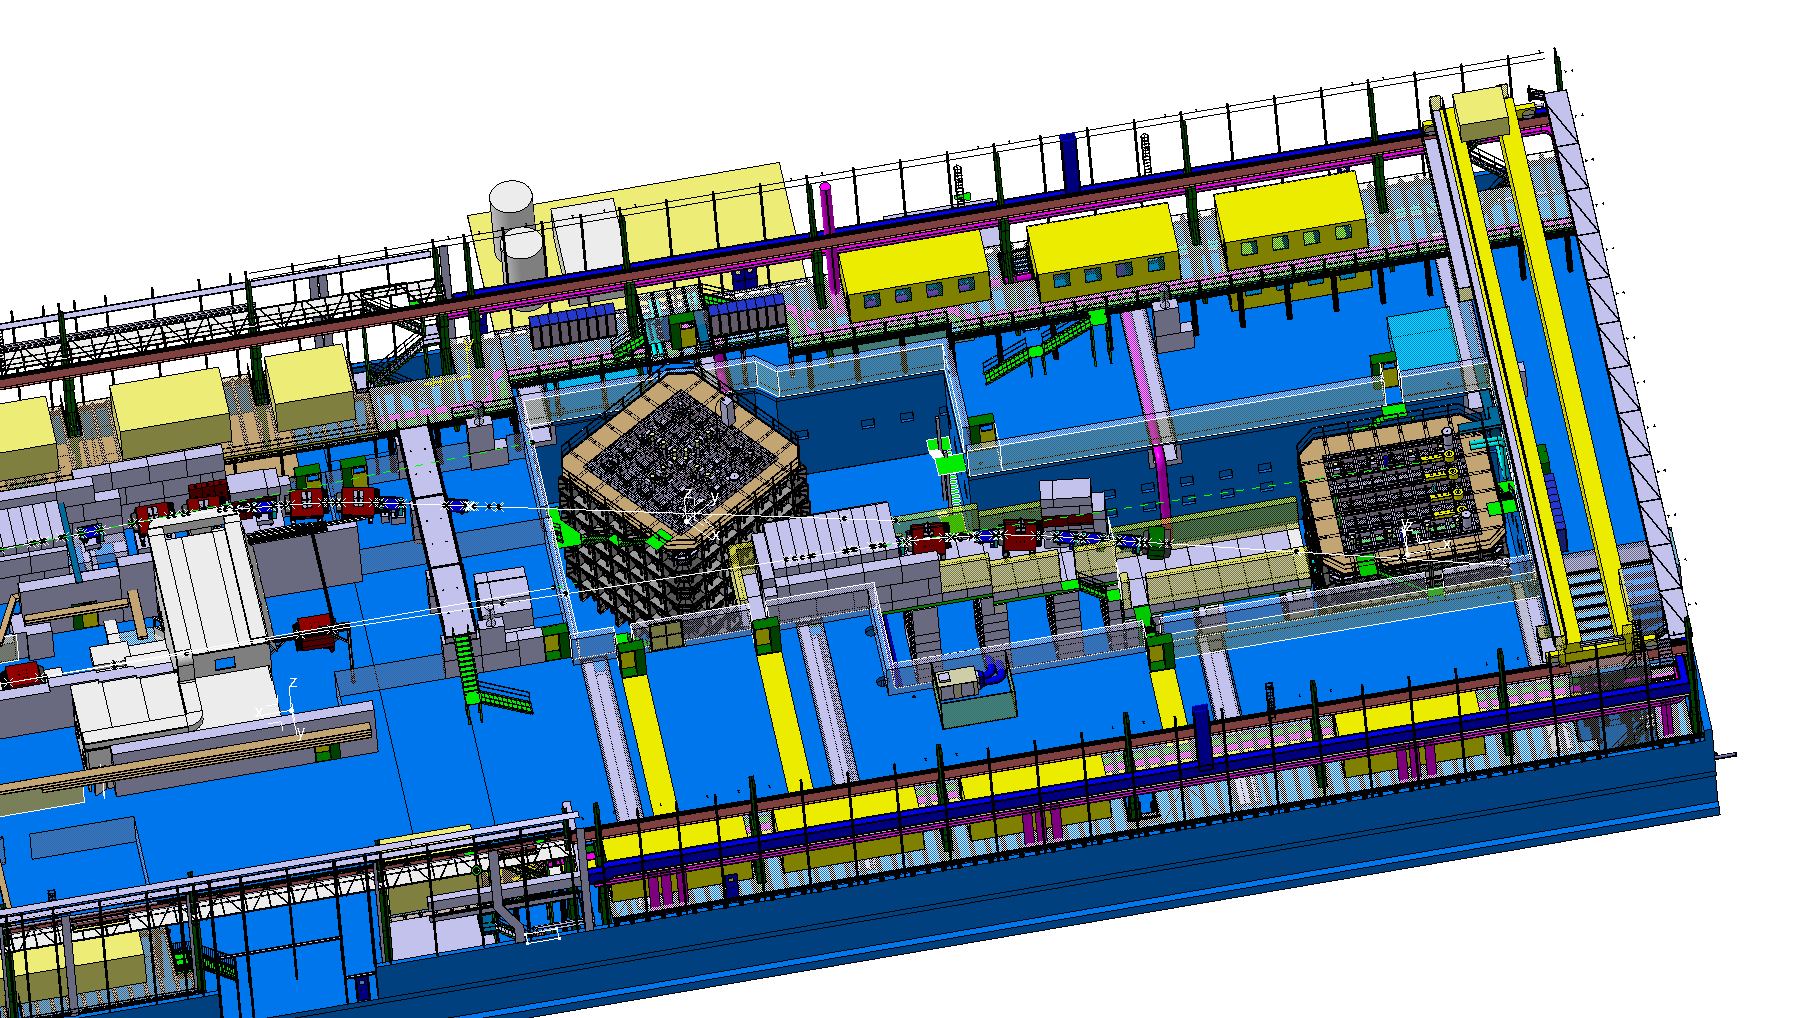
\includegraphics[width=0.8\textwidth]{figures/np02np04.png}
\caption{\label{fig:np02np04}Diagram of the layout of the CERN north area with
  staging of the protoDUNE dual phase detector (center) and single
  phase detector (right).}
\end{figure}
%%%%%%%%%%%%%%%%%%%%%%%%

\section{LArTPC as a Data Source}
\label{sec:np04_data_rate}
DUNE/\pd LArTPC design has a fine spatial resolution due to the high
channel count and spatial granularity, wire pitch and geometry, of the readout
planes.  The readout design also takes advantage the relatively slow
drift velocity of ions in the Argon and the 2~MHz digitization clock
to achieve similarly fine spatial and temporal resolution long the
drift axis of the detector, corresponding to the 5~ms drift time across
the active volume.  These characteristics are typical of
similar modern TPC detectors.

\noindent These factors do however, in the absence of zero
suppression, result in a large data volume needing to be readout and
processed for a single event (drift) trigger. for a
single considerable amount of data collected per single event readout.
A DUNE/\pd readout event may be compared to sequential stack of a thousand of digital
images of the signals collected from the electrodes. 
The instantaneous triggered data rate and the data rates averaged over
the beam's spill and duty factors are expected to be primarily limited
by the network bandwidth available within the DAQ infrastructure and
the I/O bandwidth available for recording the data.  Lossless data
reduction/compression (e.g. Huffman encoding)
techniques are applied to the data within the DAQ readout chain and
are projected to result in a factor of 4x reduction to the raw data.
Based on these projections, the NP04 experiment is expected to accumulate 2.5~PB of physics beam
data during 3 months of running.  The total data volume accumulated by
the experiment is expected to be larger when data from
detector commissioning prior to the beam run, and cosmic ray data from
after the beam running are included.   These rates are detailed in Sec.\,\ref{table:np04_data_rate}.

% \section{The NP04 Data Characteristics}
% \label{sec:np04_data_rate}
% The following nominal parameters define the expected data rates and volume in NP04:
% \begin{itemize}
% \item TPC channel count: 15,360
% \item Digitization frequency: 2MHz
% \item Readout window: 5\,ms
% \item Trigger rate: 100\,Hz
% \item SPS spill time: 4.8\,s
% \item SPS cycle: 16.8\,s
% \item Compression: $\times$4
% \end{itemize}
% \noindent This results in the following nominal data characteristics:
% \begin{itemize}
% \item Instantaneous rate (in DAQ): 11.5\,GB/s
% \item Average rate (including ingestion into mass storage): 3.3\,GB/s
% \item Total data to be captured: 6\,PB
% \item Buffer to store 3 days worth of data: 850\,TB
% \end{itemize}

\begin{table}
\begin{center}
\caption[GPS Detector Locations]{\label{table:np04_data_rate}
  Detector, beam, DAQ and data rate parameters for the single phase
  \pd experiment (NP04).}
\begin{tabularx}{0.75\textwidth}{ X  >{\setlength{\hsize}{0.8\hsize}}r}
\hline
Detector Parameter & Target \\
\hline
TPC channel count & 15,360 \\
Digitization frequency & 2~MHz \\
Readout window & 5~ms \\
SPS spill time& 4.8~s\\
SPS cycle& 22.5~s\\
Trigger rate (target minimum/maximum) & 25-100~Hz \\
Single readout size (per trigger) & 230.4~MB \\
Target compression factor& $\times$4 \\
Instantaneous data rate (in-spill) & 1440 MB/s \\
Average data rate & 576~MB/s \\
Total data recorded (beam + cosmic) & 2.5\,PB\\
Buffer to store 3 days worth of data & 300\,TB\\
\hline
\end{tabularx}
\end{center}
\end{table}


\section{Raw Data Flow in \pd}
\label{sec:raw_concept}
\subsection{DAQ and the Online Buffer}
Details of the DAQ design and Online Monitoring in \pd are outside of the scope
of this document but it is helpful to note a few details relevant for the topic at hand.

The DAQ has of a few interconnected layers of processes running on dedicated computers.
The ``outer layer'' of the system where the data is put together in a format
suitable for writing into files consists of  \textit{Event Builders}. The Event Builders
are hosted on a few machines equipped with quad 10Gbps NICs to ensure the necessary
bandwidth. Interconnectivity is provided by a high-bandwidth switch such as Brocade ICX 7750
or equivanent. Their function is to assemble complete readout frames from data
fragments obtained from the inner layer of DAQ, the \textit{Board Readers}.

The Event Builders create the necessary file-level header information and write the
resulting data  to the \textit{Online Buffer} which is attached to the \pd DAQ. 
The design of this buffer is inspired by a system sucessfully employed in ATLAS experiment
and is based on a COTS storage hardware from DELL which features a high degree of redundnacy.
It is structured as 3 identical high-capacity storage system, i.e.~scales vertically. Each system contains
\begin{itemize}

\item Two front-end nodes (DELL R620 or similar)
\item Storage Controller (DELL MD3420 or similar)
\item Four expansion shelves (DELL MD1220 or similar)
\item A total of $\sim$120 HDDs
\end{itemize}

\noindent In addition to redundancy, the high HDD count is the main factor which allows
to sink \pd data to the disk at the high rate according to the experiment plan (Sec.\,\ref{sec:np04_data_rate})
and have enough headroom for robust operation.


A backup (auxiliary) option is to implement the buffer as a a XRootD \cite{xrootd} cluster
that may be deployed on existing general purpose hardware provided by the \textit{CERN
Neutrino Platform}\cite{cenf}.
A small prototype of such system has been tested.


\subsection{The Data Flow pattern in \pd}
\label{sec:flow}
%%%%%%%%%%%%%%%%%%%%%%%%
\begin{figure}[tbh]
\centering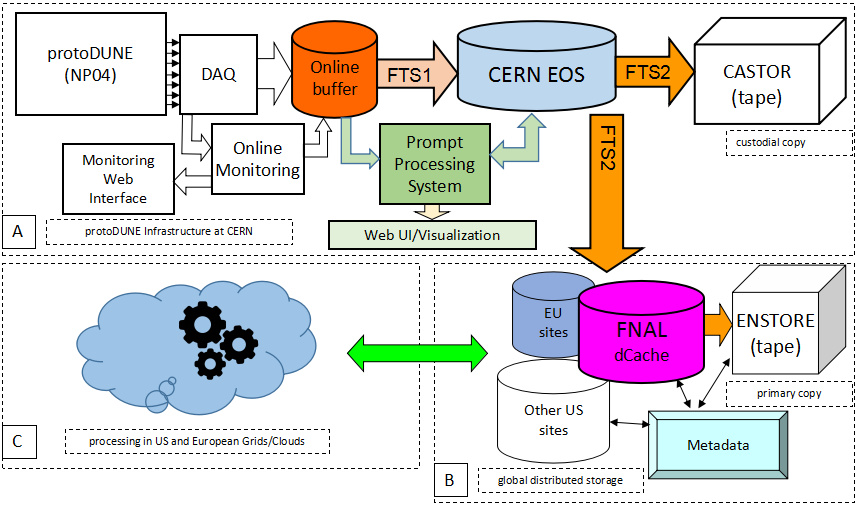
\includegraphics[width=0.85\linewidth]{figures/protoDUNE_data_flow_2017_v2.png}
\caption{\label{fig:raw_concept}Conceptual diagram of the flow of raw data in \pd}
\end{figure}
%%%%%%%%%%%%%%%%%%%%%%%%

In the following, we shall consider handling and management of the raw data after it is
written by the Event Builders to the Online Buffer.  Conceptual diagram of the raw data
flow in \pd is presented in Fig.\ref{fig:raw_concept} which shows the general pattern of data flow
and also reflects the central role of the EOS system at CERN \cite{eos} in the raw data management scheme.
Reliance on EOS is motivated by the experience and architecture of the LHC experiments
as well as the \pd data characteristics presented above in Sec.\,\ref{sec:np04_data_rate}.

The elements in this diagram which contain ``FTS'' in their label correspond to components and
instances of the \textit{Fermi File Transfer Service} -- FTS for short \cite{fts} -- which transports
data between a predefined endpoints. Fermi FTS was designed originally for NOvA experiment
\cite{nova} DAQ system and has a proven track record of moving over 7.7\,PB of data for NOvA
and 4.7\,PB of data for MicroBooNE\,\cite{uboone}.
The Fermi FTS contains functionality which allows for completely automatic operation
including error handling, transmission retries, monitoring etc.

There is more than once instance of FTS in the \pd data transmission chain. One instance (labeled ``FTS1''
in the diagram) is responsible for moving the data from the Online Buffer into EOS. The second instance
-- ``FTS2'' --  copies the data after is has arrived to EOS to tape storage at CERN (the CASTOR
system~\cite{castor}). It is also tasked with transmitting the data to Fermilab  and other peer
institutions. At FNAL the data are placed in a dCache~\cite{dcache} storage cluster. A secondary
tape copy is then created at Fermilab using the data resident in dCache as the source.
Other participating data centers receiving their copies of raw data may function differently
e.g.\,use other methods of local storage federation.

\subsection{The ``Dropbox'' Logic}
In both instances an FTS agent is triggered by arrival of files to a designated
storage location which is expected to be accessible in a POSIX-like  mode.
It effectively serves as a ``dropbox'', i.e.\,files are selected
for transfer asyncronously based on certain criteria (such as the filename pattern etc)
and subjected to following operations:
\begin{itemize}
\item Identified
\item Registered
\item Scheduled for transmission
\item Verified
\item Cleaned up after transfer
\end{itemize}


\subsection{Metadata}
An important feature of the FTS is its interface to and integration with 
the \textit{SAM} Metadata system deployed at FNAL which serves the needs of a few
experiments in both High Energy Physics and Intensity Frontier domains. In addition to essential file catalog
functionality, SAM has extensive storage management
capabilities covering both disk (e.g.\,dCache) and tape (e.g.\,FNAL Enstore) types of storage.
% Working in tandem, FTS and SAM allow
The most common way
to associate metadata with a file in SAM is to package it as an auxiliary file in JSON format,
following a certain naming convention. This file is then automatically detected by FTS
and records in SAM are created in accordance with its content.

Operations related to metadata present certain challenges in the high-volume and high-rate
environment of the \pd data flow. For example, for the metadata to be useful, it may
be necessary to extract some of its elements by reading a large fraction or even all of the data file
written to the buffer. In the very high I/O bandwidth scenario of \pd this puts substantial additional
load on storage systems. Another example is checksum operations as the checksum is often
considered a crucial part of the file metadata. If checksums are required from the very beginning
of the data transfer chain, complete files must be read from the Online Buffer. In addition, handling
checksums requires a non-negligible amount of CPU.

Current plan is to utilize the checksum calculattion capabilities provided by XRootD
during both legs of the transfer: it is first calculated by the ``FTS1'' instance
(see \ref{sec:flow}) and added as a part of the metadata. It is then used in further transfers
by ``FTS2'' to CASTOR and dCache.

\subsection{Transfer Protocols}
A number of protocols are supported by both EOS and FTS inclusing XRootD, gridFTP
and third-party transfers. Prime candidate for \pd is XRootD which has proven scalability
and reliability.

In addition to serving as the principal staging area from which the data is copied to
tape storage at CERN and from which it is transmitted to FNAL, 
EOS will also be used to provide transparent access to data to the
\pd prompt processing system 
in order support the Data Quality Moniotring (DQM) in \pd as explained in Sec.\,\ref{sec:dqm}.
Its XRootD interface makes it a particularly attractive option.

\section{Data Quality Monitoring}
\label{sec:dqm}
Data Quality Monitoring (DQM) plays an imporant role in \pd.
Its goal is to generate time-critical information on a short time
scale needed to ascertain the condition
and performance of both the detector and the DAQ,
in order for operators to quickly detect problems, take action and prevent loss
of useable data and/or beam time.

DQM consists of two parts,  the low latency Online Monitoring (OM)
system which is engineered as a component of DAQ, and
the ``prompt processing system''. This is reflected in the diagram
in Fig.\ref{fig:raw_concept}.
These systems are complementary to each other but operate
in different enviroments and on a different time scale.
The benchmark turnaround time for ``prompt processing'' jobs 
is set roughly at 10\,min, with actual numbers depending on
finalized content of the payloads. Jobs will be organized and stages
and subject to prioritization to guarantee timely production of DQM
visual and data products. A prototype system has been developed at
the time of writing. The final stages of prompt processing will
include simplified event reconstruction based on LArSoft framework
\cite{larsoft}.

Compared to prompt processing, Online Monitoring aims
to provide response on the scale of seconds and in general under a minute.
The prompt processing system processes only a small fraction of the data
but can potentially perform more sophisticated calculations since it is
easier to scale out its CPU capabilities. Both OM and prompt processing system
will be located in the vicinity of the NP04 detector. It may be necessary to
scale out parts of prompt processing to the CERN central batch facility
so the system is designed to support this mode of operation as well.

\section{Summary}
The single-phase \pd experiment will generate data at a very high rate
with a few PB of raw data to be recorded in mass storage during the time of
its operation. To meet the challenges associated with handling these
data the DUNE Collaboration opted to leverage designs, software and
components from a few HEP and Intensity Frontier experiments. This includes
\begin{itemize}
\item The design of the Online Buffer
\item The principal data transfer system (Fermi FTS) and the Metadata system (Fermilab SAM)
\item XRootD storage federation technology
\item LArSoft framework for Liquid Argon detector simulation and reconstruction
\end{itemize}

\section*{References}
\begin{thebibliography}{9}

\bibitem{cdrVol1} DUNE CDR Vol 1 -- The LBNF and DUNE Projects\\
\url{http://arxiv.org/abs/1601.05471}

\bibitem{cdrVol4} DUNE CDR Vol 4 -- The DUNE Detectors at LBNF\\
\url{http://arxiv.org/abs/1601.02984}

\bibitem{np04} 
Yearly report on ProtoDUNE Single Phase NP04 (2016)\\
\url{https://cds.cern.ch/record/2144868}

\bibitem{xrootd}
{XRootD}\\
\url{http://www.xrootd.org}

\bibitem{cenf}
{CERN Neutrino Platform}\\
\url{http://home.cern/about/experiments/cern-neutrino-platform}


\bibitem{eos}
{The CERN Exabyte Scale Storage}\\
\url{http://information-technology.web.cern.ch/services/eos-service}

\bibitem{fts}
{The Fermilab File Transfer System}\\
\url{http://cd-docdb.fnal.gov/cgi-bin/RetrieveFile?docid=5412&filename=datamanagement-changeprocedures.pdf&version=1}

\bibitem{nova}
NOvA Neutrino Experiment\\
\url{https://www-nova.fnal.gov/}

\bibitem{uboone}
MicroBooNE Neutrino Experiment\\
\url{http://www-microboone.fnal.gov/}

\bibitem{castor}
{CASTOR -- CERN Advanced STORage manager}\\
\url{http://castor.web.cern.ch/}

\bibitem{dcache}
{dCache.org}\\
\url{https://www.dcache.org/}

\bibitem{sam}
{A data handling system for modern and future Fermilab experiments}\\
\url{http://iopscience.iop.org/1742-6596/513/3/032045}

\bibitem{larsoft}
{LArSoft Collaboration}\\
\url{http://larsoft.org//}

\end{thebibliography}





\end{document}


